\documentclass[zihao=false,fontset=windows]{ctexart}
% ctexart 不接受任意 pt 选项。正文改 {10pt}，方括号里是行距。
\usepackage{scrextend}
\changefontsizes[12pt]{10pt}

\usepackage[a4paper,left=2.35cm,right=2.35cm,top=1.7cm,bottom=1.9cm]{geometry}
\usepackage{xcolor}
\usepackage{graphicx}
\usepackage{amsmath,amssymb}
\usepackage{enumitem}
\usepackage{tabularx}
\usepackage{colortbl}
\usepackage{listings}
\usepackage{hyperref}
\usepackage[most]{tcolorbox}

\definecolor{feishuText}{RGB}{31,35,41}
\definecolor{feishuBlue}{RGB}{36,91,219}
\definecolor{feishuRed}{RGB}{216,57,49}
\definecolor{feishuGray}{RGB}{100,106,115}
\definecolor{feishuGray2}{RGB}{143,149,158}
\definecolor{feishuPinkBg}{RGB}{251,191,188}
\definecolor{quoteBar}{RGB}{51,112,255}
\definecolor{codebg}{RGB}{245,246,247}
\definecolor{codeborder}{RGB}{222,224,227}
\definecolor{inlinebg}{RGB}{242,243,245}
\definecolor{callRed}{RGB}{253,226,226}
\definecolor{callOrange}{RGB}{255,245,235}
\definecolor{callYellow}{RGB}{254,255,240}
\definecolor{callGreen}{RGB}{240,251,239}
\definecolor{callBlue}{RGB}{240,244,255}
\definecolor{callRedSoft}{RGB}{254,241,241}
\definecolor{callSun}{RGB}{255,255,204}
\definecolor{tableHead}{RGB}{242,243,245}
\definecolor{tableRule}{RGB}{222,224,227}
\definecolor{codeText}{RGB}{31,35,41}
\definecolor{codeKeyword}{RGB}{0,0,255}
\definecolor{codeComment}{RGB}{0,128,0}
\definecolor{codeString}{RGB}{163,21,21}

\setmainfont{Times New Roman}
\setCJKmainfont{Microsoft YaHei}[AutoFakeBold=2.2]
\setCJKsansfont{Microsoft YaHei}[AutoFakeBold=2.2]
\setCJKmonofont{Microsoft YaHei}[AutoFakeBold=2.2]
\setmonofont{Consolas}
\newfontfamily\emojifont{Segoe UI Emoji}

\hypersetup{
  colorlinks=true,
  urlcolor=feishuBlue,
  linkcolor=feishuBlue,
  unicode=true,
  pdftitle={LLaVA-1.5(2023, Microsoft Research)}
}

\setlength{\parindent}{0pt}
\setlength{\parskip}{0.42em}
\setlength{\fboxsep}{1.5pt}
\setlength{\emergencystretch}{3em}
\linespread{1.28}
\color{feishuText}
\arrayrulecolor{tableRule}
\urlstyle{same}

\setlist[enumerate]{label=\textcolor{feishuBlue}{\arabic*.}, leftmargin=1.7em, itemsep=0.22em, topsep=0.28em, parsep=0.08em, partopsep=0pt}
\setlist[itemize,1]{label=\textcolor{feishuBlue}{\textbullet}, leftmargin=1.35em, itemsep=0.18em, topsep=0.25em, parsep=0.06em, partopsep=0pt}
\setlist[itemize,2]{label=\textcolor{feishuBlue}{◦}, leftmargin=1.45em, itemsep=0.12em, topsep=0.15em}
\setlist[itemize,3]{label=\textcolor{feishuBlue}{\rule[0.18em]{0.38em}{0.38em}}, leftmargin=1.55em, itemsep=0.1em, topsep=0.12em}

\newcommand{\feiEmoji}[1]{{\emojifont #1}}
\newcommand{\incode}[1]{\colorbox{inlinebg}{\ttfamily\small #1}}
\newcommand{\bigmath}[1]{%
  \begin{center}\large$\displaystyle #1$\end{center}%
}

\lstset{
  language=Python,
  basicstyle=\ttfamily\footnotesize\color{codeText},
  keywordstyle=\color{codeKeyword},
  commentstyle=\color{codeComment},
  stringstyle=\color{codeString},
  showstringspaces=false,
  breaklines=true,
  columns=fullflexible,
  keepspaces=true,
  tabsize=4,
  upquote=true,
  aboveskip=2pt,
  belowskip=0pt,
  xleftmargin=0pt,
  frame=none
}

\tcbset{
  feishubase/.style 2 args={
    enhanced,
    boxrule=0pt,
    arc=8pt,
    left=10pt,
    right=10pt,
    top=7pt,
    bottom=7pt,
    before skip=6pt,
    after skip=6pt,
    colback=#1,
    colframe=#1,
    before upper={\feiEmoji{#2}\hspace{0.45em}\ignorespaces}
  }
}
\newtcolorbox{feishubox}[2]{feishubase={#1}{#2}, breakable}
\newtcolorbox{feishuboxnb}[2]{feishubase={#1}{#2}}

\newtcolorbox{feishuquote}{
  enhanced,
  breakable,
  boxrule=0pt,
  leftrule=3pt,
  arc=0pt,
  colframe=quoteBar,
  colback=white,
  left=8pt,
  right=2pt,
  top=2pt,
  bottom=2pt,
  before skip=4pt,
  after skip=4pt,
  before upper=\color{feishuGray}
}

\newtcolorbox{feishucode}{
  enhanced,
  breakable,
  colback=codebg,
  colframe=codeborder,
  boxrule=0.6pt,
  arc=6pt,
  left=6pt,
  right=6pt,
  top=5pt,
  bottom=4pt,
  before skip=6pt,
  after skip=6pt
}

\usepackage{needspace}
\definecolor{paperCite}{RGB}{0,200,125}
\definecolor{paperYellow}{RGB}{255,255,100}
% Source: https://scnajei2ds6y.feishu.cn/wiki/HTJVw44IJibX6gkYWtlc1zCYnVh
% Figures from normal browser preview screenshots; figure 3 lower text/formula transcribed into native TeX.
\begin{document}
{\zihao{1}\bfseries LLaVA-1.5(2023, Microsoft Research)\par}

% source-block: SmS4dHqbmoa6sgxGEXgcwsjinyn
\begin{feishuboxnb}{callOrange}{🙋‍♀}
论文：《Improved Baselines with Visual Instruction Tuning》\par
论文地址：\url{https://arxiv.org/pdf/2310.03744}\par
项目地址：\url{https://github.com/haotian-liu/LLaVA}\par
\end{feishuboxnb}
% source-block: WQW0dM36DokepSxV8bHcC5junHh
相比\href{https://scnajei2ds6y.feishu.cn/wiki/BNWJwSLQiizLZqkoQRtc4Pc5nPj}{LLaVA(2023, Microsoft)}主要做了几点优化：\par
% source-block: QrzedSuLSoFOkIxiMD8c1B5YnXf
\begin{itemize}
\item 使用单一的响应格式提示语，明确指示输出格式。例如，“Answer the question using a single word or phrase.”这样的提示语可以促使 LLM 根据用户的指示正确调整输出格式。
% source-block: Gy9nd3uDeo6XCzxRxTwc5rJYnuh
\item vision-language 的 connector 使用一个两层的 MLP
% source-block: Xhc2dqm92oFaddx9Ph1cHVbfnPh
\item 额外使用一些学术任务导向的数据集
% source-block: Fx4kdZsM2oagoexrWvfcVPBwngg
\item 扩大 LLM 的参数规模、图像的分辨率等
\end{itemize}
% source-block: M1yXdipczoKYcbxEZ73cO3sen2d
\Needspace{5\baselineskip}\par\vspace{1.15em}\noindent{\zihao{-2}\bfseries \textcolor{feishuBlue}{1.} 模型架构}\par\vspace{0.28em}
% source-block: PVNGdwWcDo4FLJxLEL1c09cXnXe
\begin{center}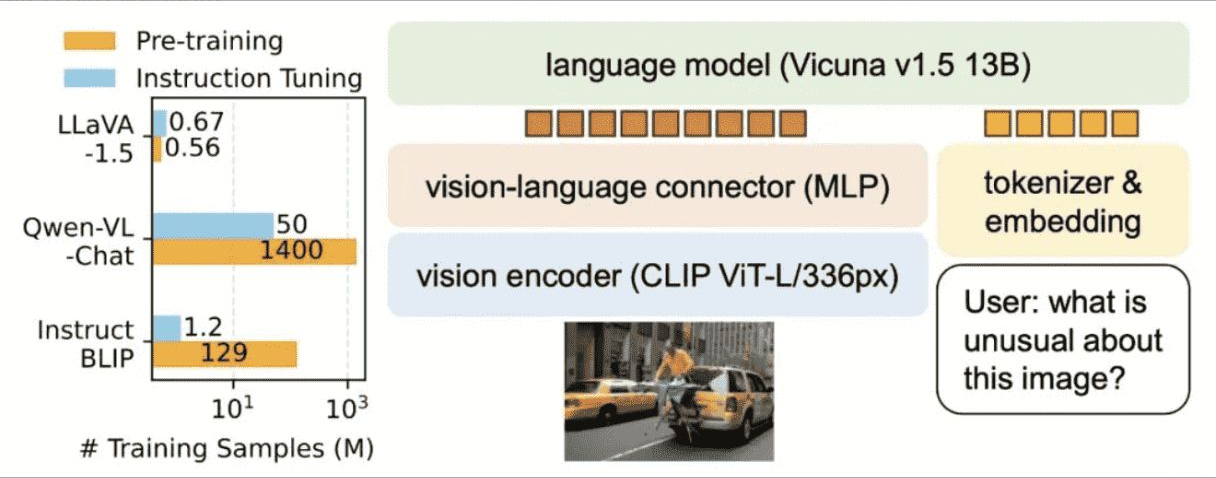
\includegraphics[width=0.98\textwidth]{images/2023-LLaVA-1.5/fig-01.png}\end{center}
% source-block: CD4EdrHfZowsNPxwUwqczLgfnpd
\Needspace{4\baselineskip}\par\vspace{0.95em}\noindent{\zihao{3}\bfseries \textcolor{feishuBlue}{1.1} Visual Encoder}\par\vspace{0.28em}
% source-block: EN0od68VkonKqkx9425cBsgLnxg
CLIP-ViT-L-14 (224\textasciicircum{}2)\par
% source-block: GxmydNhgDoN1rrxsKuecLxlonLU
CLIP-ViT-L-336px (336\textasciicircum{}2)\par
% source-block: LcAddDh5voUU2xxnKUNcFLjdncO
使用了Dynamic High-Resolution策略，用于保留高分辨率图像的细节：\par
% source-block: R6uPdYLX0ozMYTxmO0Rcl6Dzn2c
\begin{center}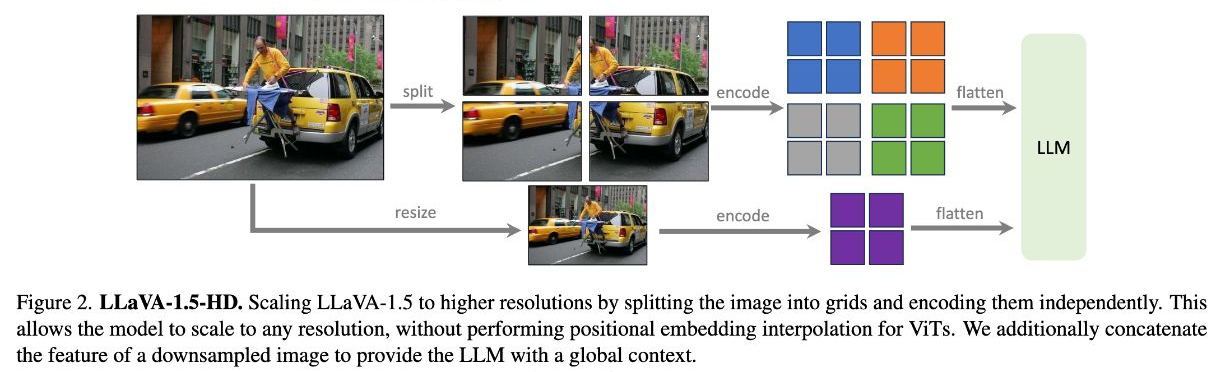
\includegraphics[width=0.98\textwidth]{images/2023-LLaVA-1.5/fig-02.png}\end{center}
% source-block: NYcDdzkF7oTwEfxrOPocZkYcnye
\begin{feishuboxnb}{callOrange}{🙋‍♀}
注意一个细节，就是LLaVA使用的ViT特征和\href{https://scnajei2ds6y.feishu.cn/wiki/AZiVwFmXEirI77kAVzYcOMNVnbh}{BLIP-2(2023, Salesforce Research)}一样，是倒数第二层。这可能因为 CLIP 的最后一层特征可能比它之前的层更关注全局和抽象的图像属性，而它之前的层可以更关注有助于理解特定图像细节的局部属性\par
\end{feishuboxnb}
% source-block: TpnXdjAceo9hwIxFh7BcRhkenLJ
这个细节可以参考\href{https://scnajei2ds6y.feishu.cn/wiki/BNWJwSLQiizLZqkoQRtc4Pc5nPj}{LLaVA(2023, Microsoft)}论文：\par
% source-block: T6JGd5vDZoax2ExcQXkcVlJinpe
\begin{center}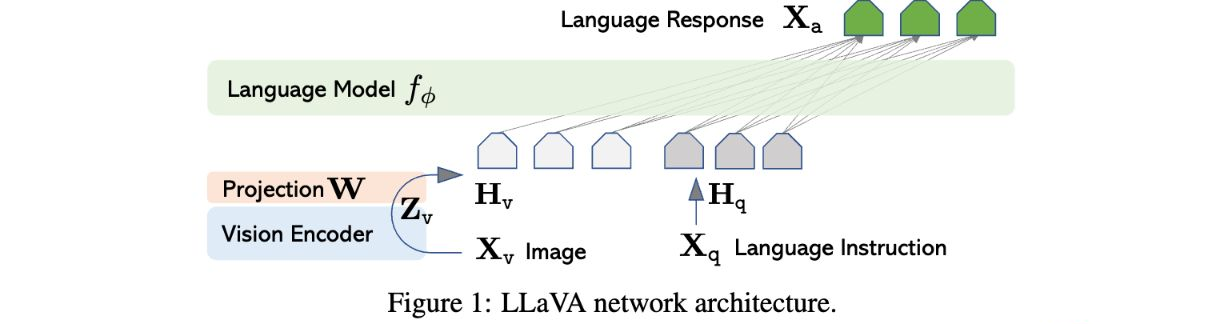
\includegraphics[width=0.98\textwidth]{images/2023-LLaVA-1.5/fig-03.png}\end{center}
% The following English paragraph and equation are transcribed from the lower half of source figure 3.
For an input image $\mathbf{X}_v$, we consider the pre-trained CLIP visual encoder ViT-L/14 \textcolor{paperCite}{[40]}, which provides the visual feature $\mathbf{Z}_v=g(\mathbf{X}_v)$. The grid features before and after the \colorbox{paperYellow}{last} Transformer layer are considered in our experiments. We consider a simple linear layer to connect image features into the word embedding space. Specifically, we apply a trainable projection matrix $\mathbf{W}$ to convert $\mathbf{Z}_v$ into language embedding tokens $\mathbf{H}_v$, which have the same dimensionality as the word embedding space in the language model:\par
{\large
\begin{equation*}
\mathbf{H}_v=\mathbf{W}\cdot\mathbf{Z}_v,\quad\text{with}\quad\mathbf{Z}_v=g(\mathbf{X}_v)\tag{1}
\end{equation*}
}
% source-block: LVHPdbKK9obZgoxO6PCcmTadnTf
\begin{feishuquote}
论文中的grid features就是features的意思，只是说ViT会分割成patch，因此叫“grid features”\par
\end{feishuquote}
% source-block: BGUjddUhOoPZKzxaGCzc42adneS
并且\href{https://scnajei2ds6y.feishu.cn/wiki/BNWJwSLQiizLZqkoQRtc4Pc5nPj}{LLaVA(2023, Microsoft)}还做了一个消融实验证明倒数第二层会更好：\par
% source-block: SFo7db8bXoP0kCxLQXTcbNdznlg
\begin{center}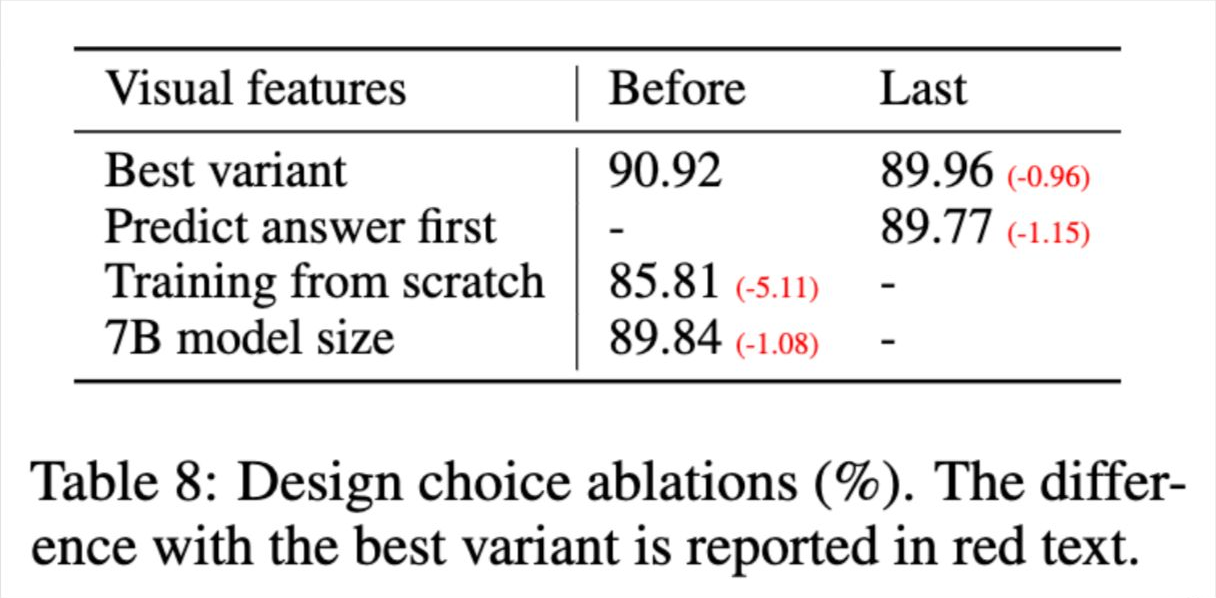
\includegraphics[width=0.98\textwidth]{images/2023-LLaVA-1.5/fig-04.png}\end{center}
% source-block: I8pqdjpGdobgIkxXc8DcEAlUn1b
\Needspace{4\baselineskip}\par\vspace{0.95em}\noindent{\zihao{3}\bfseries \textcolor{feishuBlue}{1.2} Adapter}\par\vspace{0.28em}
% source-block: PcTEd0SgRoIt4GxOddycOkjence
two-layer MLP，并且实验证明会比a linear projection表现要好\par
% source-block: ZHHpdpIQsoVUwfxG16kcGVW3nrf
\Needspace{8\baselineskip}\par\vspace{0.95em}\noindent{\zihao{3}\bfseries \textcolor{feishuBlue}{1.3} LLM}\par\vspace{0.28em}
% source-block: QdfSdKwnao1m62xlwfbcXFQqnuh
LLM语言模型升级为Vicuna v1.5 13B，语言模型参数量更大，效果更好\par
% source-block: Elh6dYWLnoH2MUxOdRecMsLCnVg
消融实验还测试了以下模型：\par
% source-block: RQq2dh8TSoWpJ3xrSgicE5YlnGc
LLaMA-based (Vicuna-v1.1, Vicuna-v1.3) \par
% source-block: GNlOdw4AjoUgy6xVdlHcbRk3nuc
LLaMA2-based (Vicuna-v1.5, LLaMA-2-Chat\par
% source-block: P5qKdlp1wokrSDxWs7Jck8SLnZC
\Needspace{5\baselineskip}\par\vspace{1.15em}\noindent{\zihao{-2}\bfseries \textcolor{feishuBlue}{2.} 模型训练}\par\vspace{0.28em}
% source-block: WfwIddGN3ozk5txmb0pcobbynpe
数据上使用了\href{https://scnajei2ds6y.feishu.cn/wiki/YJhWwVYCyiqdEMkUsWIcovFun3b}{InstructBLIP(2023, Salesforce Research)}使用的：\par
% source-block: M1GKdZKAWoCdD7x1QTDcU1Tvncc
\begin{itemize}
\item VQA (OKVQA, A-OKVQA) 
% source-block: EVB0dAbKtoc2OFxBzi9c19IMnqg
\item OCR (OCRVQA, TextCaps)
\end{itemize}
% source-block: GBhZdNloDouXNRxIOiDcRBz1nNf
以及region-level VQA datasets\par
% source-block: S8oddmDTboRLcfxusGmcwaRhn8c
\begin{itemize}
\item Visual Genome
% source-block: Zfmodsw9VoJYbix4hMgc0jpwnAd
\item RefCOCO
\end{itemize}
% source-block: PcBBdVuNvoS9pJxOcPMcwpycnjg
训练模式参考\href{https://scnajei2ds6y.feishu.cn/wiki/BNWJwSLQiizLZqkoQRtc4Pc5nPj}{LLaVA(2023, Microsoft)}两阶段训练。\par
% source-block: TwkRdZrRtoGq0kxZjI2cOxe0n3d
模型在三个维度上scaling的效果：\par
% source-block: TQ7ldy4a3oTnj8xnP3pcyVcGnTf
\begin{center}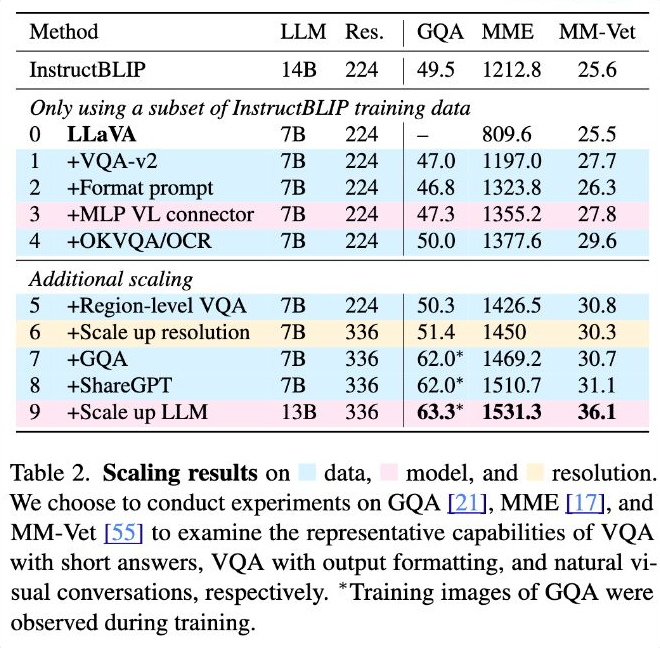
\includegraphics[width=0.92\textwidth]{images/2023-LLaVA-1.5/fig-05.png}\end{center}
\end{document}
